\subsection{Experimental setup}
The experiments were executed in a Mac Book Pro with the following characteristics: 2,6 GHz Intel Core i5, 8 GB 1600 MHz DDR3 memory and 256 GB of storage.

\subsection{Analysis}
Data set coming from previous steps are used as an input for the calculations in the analysis. These are some of the most relevant features:
\begin{itemize}
    \item system\_time - timestamp of the recording
    \item cell\_loc - event's approximated location
    \item gps\_loc - event's GPS location, considered as ground truth
\end{itemize}

The analysis phase is executed with a following steps. For each date between 2018-03-12 and 2018-03-16 we do the following:
\begin{enumerate}
    \item Import input data from Parquet files
    \item Calculate Euclidean distance measure on trajectories
    \item Calculate edit distance distance measure on trajectories
\end{enumerate}

For the whole input data set we also do the following:
\begin{enumerate}
   \item Generate and display histograms on pairwise distances
    \item Calculate descriptive statistics on pairwise distances:
        \begin{itemize}
            \item min
            \item max
            \item sum
            \item mean
            \item standard deviation
        \end{itemize}
    \item Visualize on map
\end{enumerate}
    
\subsection{Results}
Looking at the histogram of pairwise spatial distances between the trajectories in Figure\ref{fig:hist} we can say that there are three larger groups. There are slightly more events that were positioned between 200 and 250 meters accuracy, than events positioned with accuracy between 500 and 1000 meters. Almost the same number of events were however positioned with more than 5000 meters accuracy.

We expect that the quality of positioning can be significantly improved by using more accurate and robust information about cell towers.

\begin{figure}[h]
    \centering
    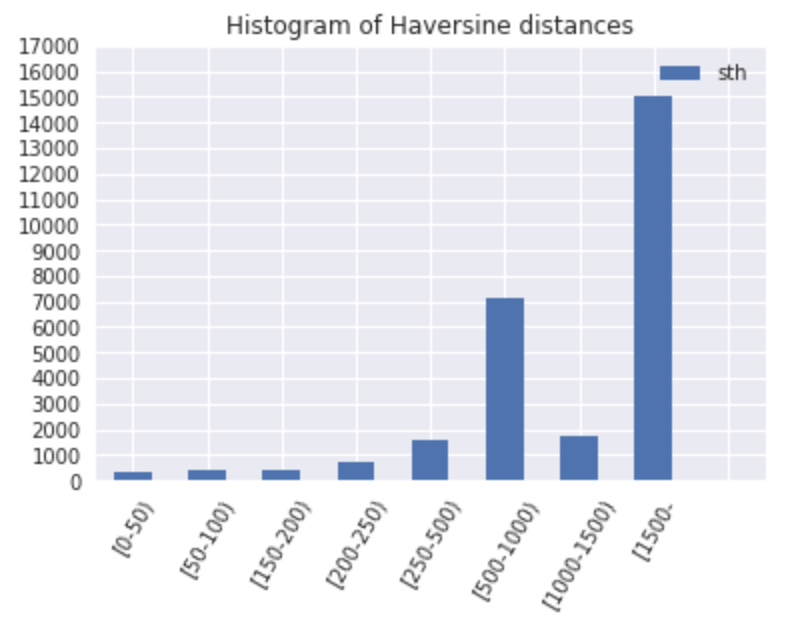
\includegraphics[width=0.5\textwidth]{images/hist.png}
    \caption{Histogram of pairwise spatial distance of the point in trajectories}
    \label{fig:hist}
\end{figure}

This result can change depending on individual customer's mobile usage habits, network characteristics, cell map data source and the customer's geographical position.

As seen in Table \ref{tab:dist_stats}, there are only 2780 CDR observations, which were successfully positioned out of 37062 observations between 2018-03-12 and 2018-03-16. This 7.5\% positioning ratio is lower than expected and indicates that most of the cell IDs that were recorded by the application can not be found in the cellmap. This is likely to be because of the fact that the cellmap's quality is poor.

We see the maximum distance is more than 8 kilometers, which seems to be quite high given we only had observations within the city of Berlin, where we did not expect distances larger than 2-3 kilometers because the cells are usually smaller in the urban area \cite{cell-site}. This can also support the argument that the quality of the cellmap is poor.

The average distance is around 2 kilometers, with a very high (2 kilometers) standard deviation. Therefore we can say that the distances are very volatile, which can be because of the fact that the user moves around with the test phone and when it is closer to the cell site the distance is very low and as the user moves farther away the distance becomes larger.

From Figure\ref{fig:traj}, we can conclude that the overall positioning needs a lot of improvement. 

\begin{figure}[h]
    \centering
    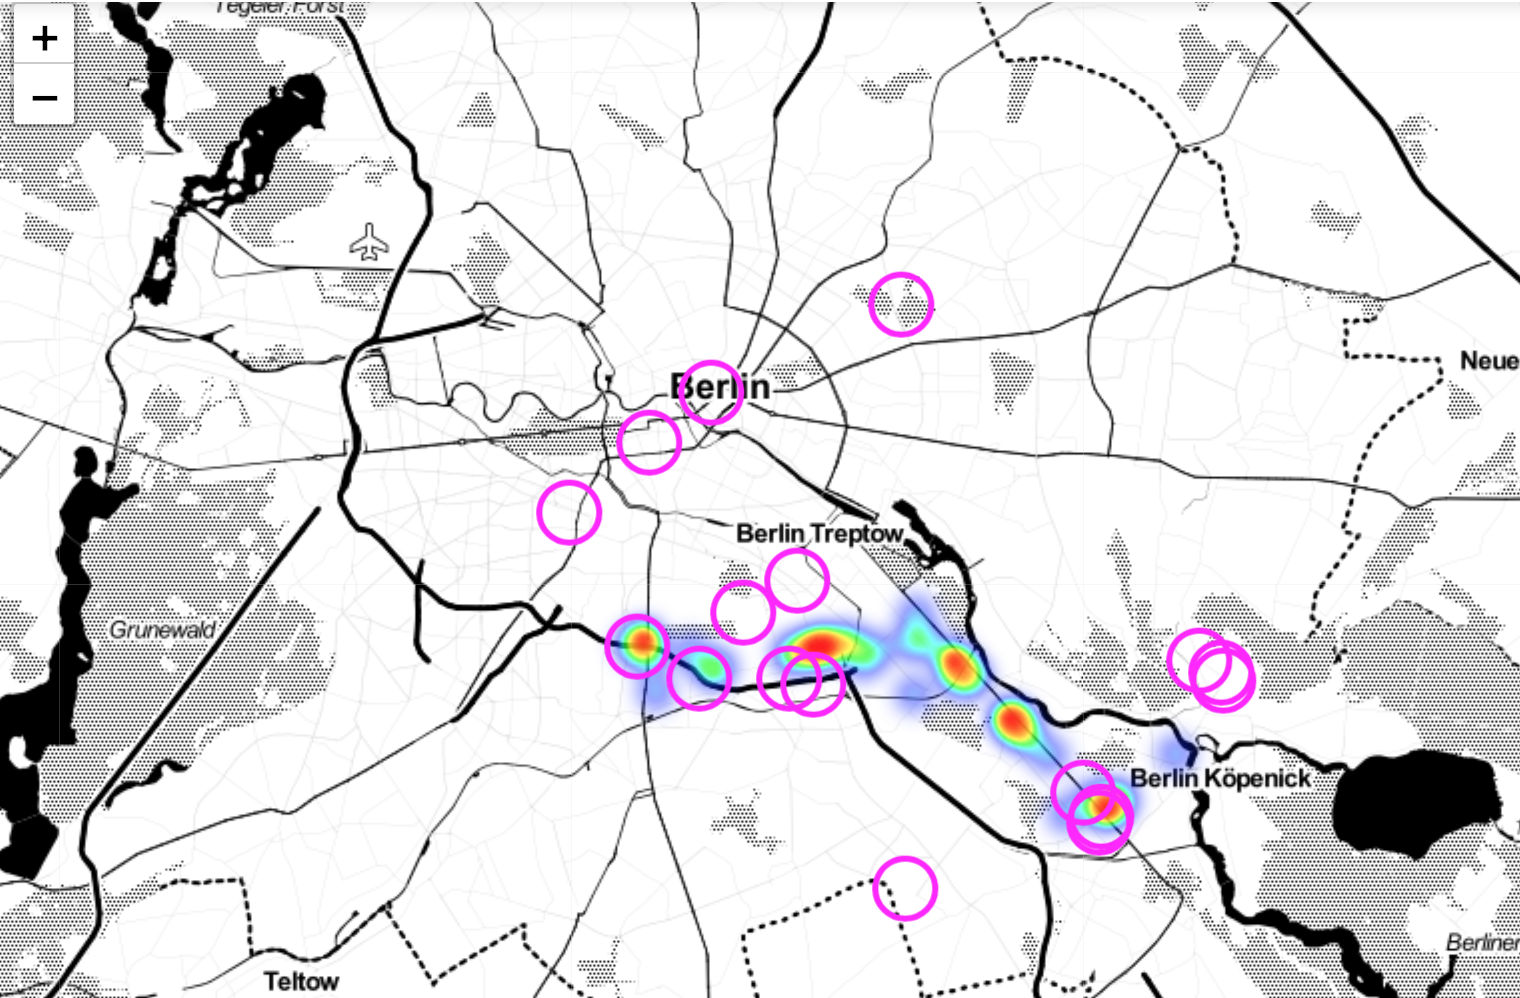
\includegraphics[width=0.5\textwidth]{images/traj.png}
    \caption{Localized CDR observations with GPS ground truth.\textit{Legend}: magenta circle marker shows the CDR observations positioned with Opencellid Cellmap and heatmap represents GPS records}
    \label{fig:traj}
\end{figure}

Euclidean distance tends to penalize large distances thus the high values seen in Table \ref{tab:distances}. The absolute values of the two types of distances cannot be compared, as their measure is different. The Euclidean distance grows with the number of events, but the edit distance does not. 

The Euclidean distance is measured in meters, therefore it is simple to interpret and scales well with the number of observations. It is also very easy to implement with pySpark DataFrames. In contrast with this, the result of edit distance algorithm has not direct interpretation and its time complexity and the nature of the algorithm makes it significantly slower. Due to the fact that it is a dynamic programming problem, it is also not straightforward to implement as pySpark DataFrame operations.

\begin{table}[h]
    \centering
    \begin{tabular}{|l|c|}
        \hline
        \textbf{Statistic} & \textbf{Value} \\
        \hline 
        count & $2780$ \\
        \hline
        min(dist) &  $49.57$\\
        \hline
        max(dist) &   $8361.66$\\
        \hline
        avg(dist) &  $2255.51$\\
        \hline
        stddev(dist) &  $2807.06$\\
        \hline
    \end{tabular}
    \caption{Descriptive statistics of Haversine distances (in meters) for target period}
    \label{tab:dist_stats}
\end{table}


\begin{table}[h]
    \centering
    \begin{tabular}{|l|c|c|c|}
        \hline
        \textbf{date} & \textbf{euc\_dist} & \textbf{edit\_dist} & \textbf{count}\\
        \hline
        2018-03-12 & 35512.63 & 5001.99 & 274 \\
        \hline
        2018-03-13 & 96574.81 & 4217.92 & 800 \\
        \hline
        2018-03-14 & 87555.24 & 3594.97 & 472 \\
        \hline
        2018-03-15 & 100162.46 & 2766.2 & 538 \\
        \hline
        2018-03-16 & 88055.91 & 4863.57 & 696 \\
        \hline
    \end{tabular}
    \caption{Distance measures for dates in the studied period}
    \label{tab:distances}
\end{table}

When the user is located between several cell towers, the connection can be passed from one tower to another depending on network traffic fluctuations and other factors. This phenomenon is often referred to as cell tower ping-pong handover. It can however be used for improving positioning and identifying points-of-interest (POIs). As seen in Figure \ref{fig:ping-pong}, the phone connects to a cell tower and to another one and then back again to the previous one. Without knowing the actual GPS position we could better approximate the location of the customer using the ping-pong handover schema.

\begin{figure}[h]
    \centering
    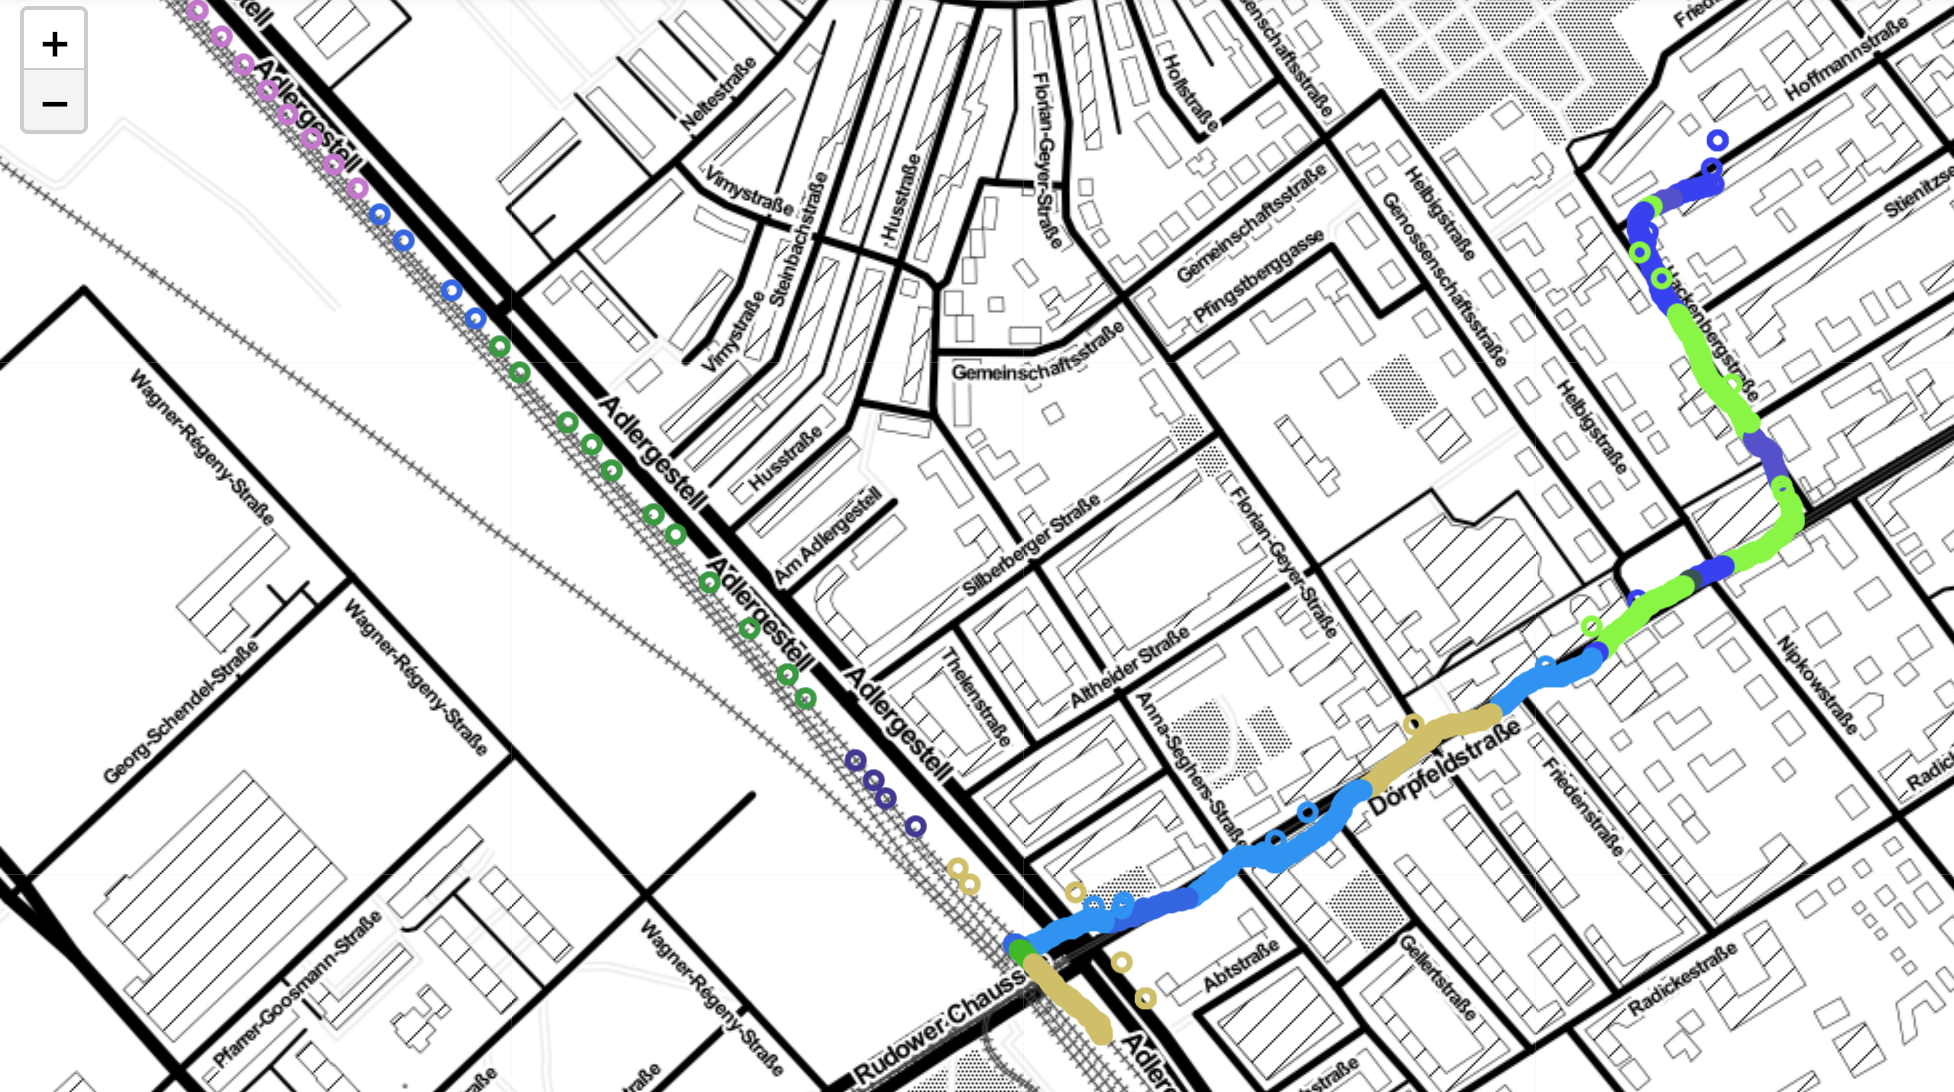
\includegraphics[width=0.5\textwidth]{images/ping-pong.png}
    \caption{Cell ping-pong handover problem, GPS points color based on the connected cell tower}
    \label{fig:ping-pong}
\end{figure}

This method can be further improved if we take into account the angle of the antennas on the cell towers. If we know which antenna is getting the signal, we can guess the direction of the transmitting cell phone and the signal strength can give an approximation of how far away it is. This method is called cell tower triangulation and can be quite accurate in rural regions with more cell towers. However the information about the angles of the antennas and the signal strength can be outdated or even missing therefore it is not always applicable. In this analysis we did not obtain robust data about the positions of the antennas and the signal strength for each CDR event.

Positioning could be improved by reconstructing trajectories considering the road network of Berlin and the potential speed of the movement instead of simply assigning the the cell location from the cell map data.

We identified three major external factors defining the accuracy of the positioning:
\begin{itemize}
    \item individual mobile usage habits affecting the sparsity of CDR data,
    \item geographical location, as rural and urban areas has different cell size and therefore location defines the accuracy of cell tower localization and
    \item cellular network characteristics that define the overall data quality and the available attributes in the CDR data-set.
\end{itemize}
